% VUT FIT MITAI
% MSZ 2021/2022
% Author: Vladimir Dusek
% Login: xdusek27

%%%%%%%%%%%%%%%%%%%%%%%%%%%%%%%%%%%%%%%%%%%%%%%%%%%%%%%%%%%%%%%%%%%%%%%%%%%%%%%%

% Path to figures
\graphicspath{{pds/teorie_smerovani/figures}}

%%%%%%%%%%%%%%%%%%%%%%%%%%%%%%%%%%%%%%%%%%%%%%%%%%%%%%%%%%%%%%%%%%%%%%%%%%%%%%%%

\chapter{PDS~--~Metody pro výpočet směrování v sítích (Bellman-Ford, Dijkstra, Path vector, DUAL).}

% todo:
% typy komunikace: broadcast, multicast, unicast
% jak algoritmy detekuji smycky ("smerovaci smycky")

%%%%%%%%%%%%%%%%%%%%%%%%%%%%%%%%%%%%%%%%%%%%%%%%%%%%%%%%%%%%%%%%%%%%%%%%%%%%%%%%

\section{Zdroje}

\begin{compactitem}
    \item \path{09-teorie-smerovani.pdf}
    \item \path{PDS_2021-04-16.mp4}
\end{compactitem}

%%%%%%%%%%%%%%%%%%%%%%%%%%%%%%%%%%%%%%%%%%%%%%%%%%%%%%%%%%%%%%%%%%%%%%%%%%%%%%%%

\section{Směrování}

Z pohledu směrování můžeme počítačovou síť zjednodušit na neorientovaný, ohodnocený graf, kde uzly jsou směrovače a hrany jsou propojení mezi něma. Směrování je pak hledání nejkratší cesty mezi dvěma uzly, resp. ze zdrojového do všech.

\paragraph*{Autonomní systém} Není možné směrovat přes celý internet (příliš velký, příliš mnoho uzlů). Využíváme abstrakce, kdy se na podsíť díváme jako na uzel~--~tzv. autonomní systém. Tímto agregujeme více informací do jedné (přesné adresy uzlů, na vyšší úrovni reprezentujeme pouze adresou sítě). Internet je pak síť sítí. Může být více úrovní (autonomní systém autonomních systémů).

\paragraph*{Hierarchické směrování} Hierarchické směrování znamená, že nesměrujeme mezi každým směrovačem na světě, ale využíváme autonomní systémy. Směrujeme tedy globálně mezi autonomníma systémama a pak uvnitř mezi směrovačema.

\begin{figure}[H]
    \centering
    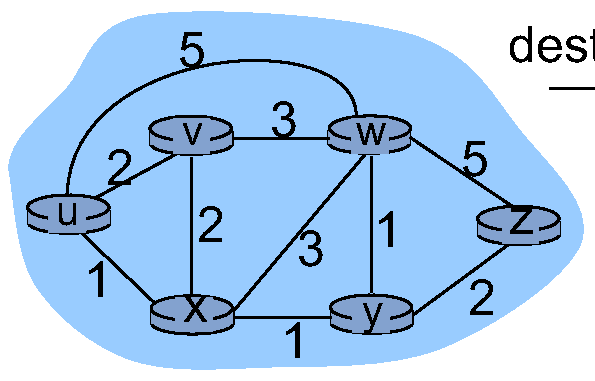
\includegraphics[width=0.5\linewidth]{network_abstraction.pdf}
    \caption{Příklad počítačové sítě zobrazené jako neorientovaný ohodnocený graf $G=(V, E)$, $V=\{u, v, w, x, y, z\}$, $E = \{ (u, v), \dots \}$, $w = \{ ((u, v), 2), \dots \}$.}
\end{figure}

\begin{figure}[H]
    \centering
    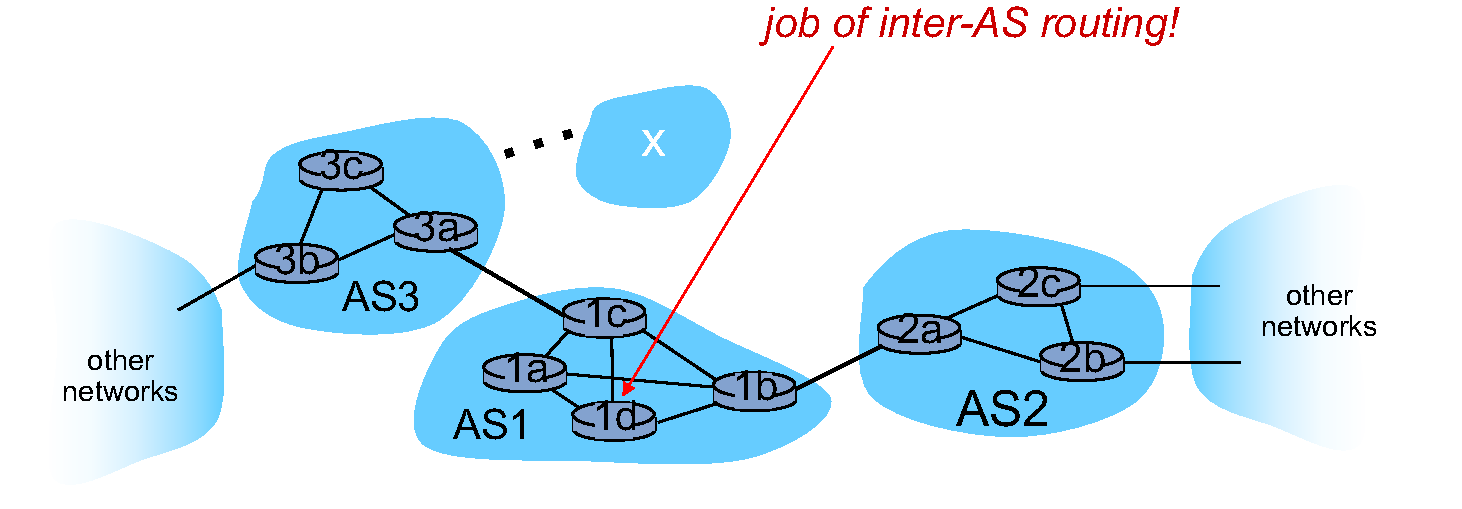
\includegraphics[width=1\linewidth]{autonomni_systemy.pdf}
    \caption{Příklad autonomních systémů (např. VUT, CESNET, UPC, \dots).}
\end{figure}

%%%%%%%%%%%%%%%%%%%%%%%%%%%%%%%%%%%%%%%%%%%%%%%%%%%%%%%%%%%%%%%%%%%%%%%%%%%%%%%%

\section{Distance Vector přístup}

\begin{compactitem}
    \item Distribuované směrovací informace~--~Každý uzel, zná pouze omezenou část topologie sítě. Konkrétně má informace pouze co sám zná a informace od svých sousedů.
    \item Používá se pro směrování uvnitř autonomních systémů.
    \item \textit{Single-metric}.
\end{compactitem}

\subsection{Algoritmus Bellman-Ford}

\begin{compactitem}
    \item \textit{Pro formální vysvětlení a pseudokód viz otázku \uv{Hledání nejkratších cest ze zdrojového uzlu do všech ostatních uzlů grafu}.}
    \item Jde o algoritmus hledání nejkratších cest ze zdrojového uzlu do všech ostatních uzlů. To znamená, že ho provádí každý uzel (směrovač).
    \item Využívá jej např. směrovací protokol RIP (\textit{Routing Protocol}). \begin{compactitem}
        \item Komunikuje přes UDP na portu 520.
        \item Metrika: \textit{hop count}.
        \item Proti \textit{Infinity Count} (viz dále) se brání vylepšením \textbf{Split Horizon}: Nikdy se nepošle informace o cestě zpátky rozhraním, ze kterého přišla.
    \end{compactitem}
\end{compactitem}

\begin{figure}[H]
    \centering
    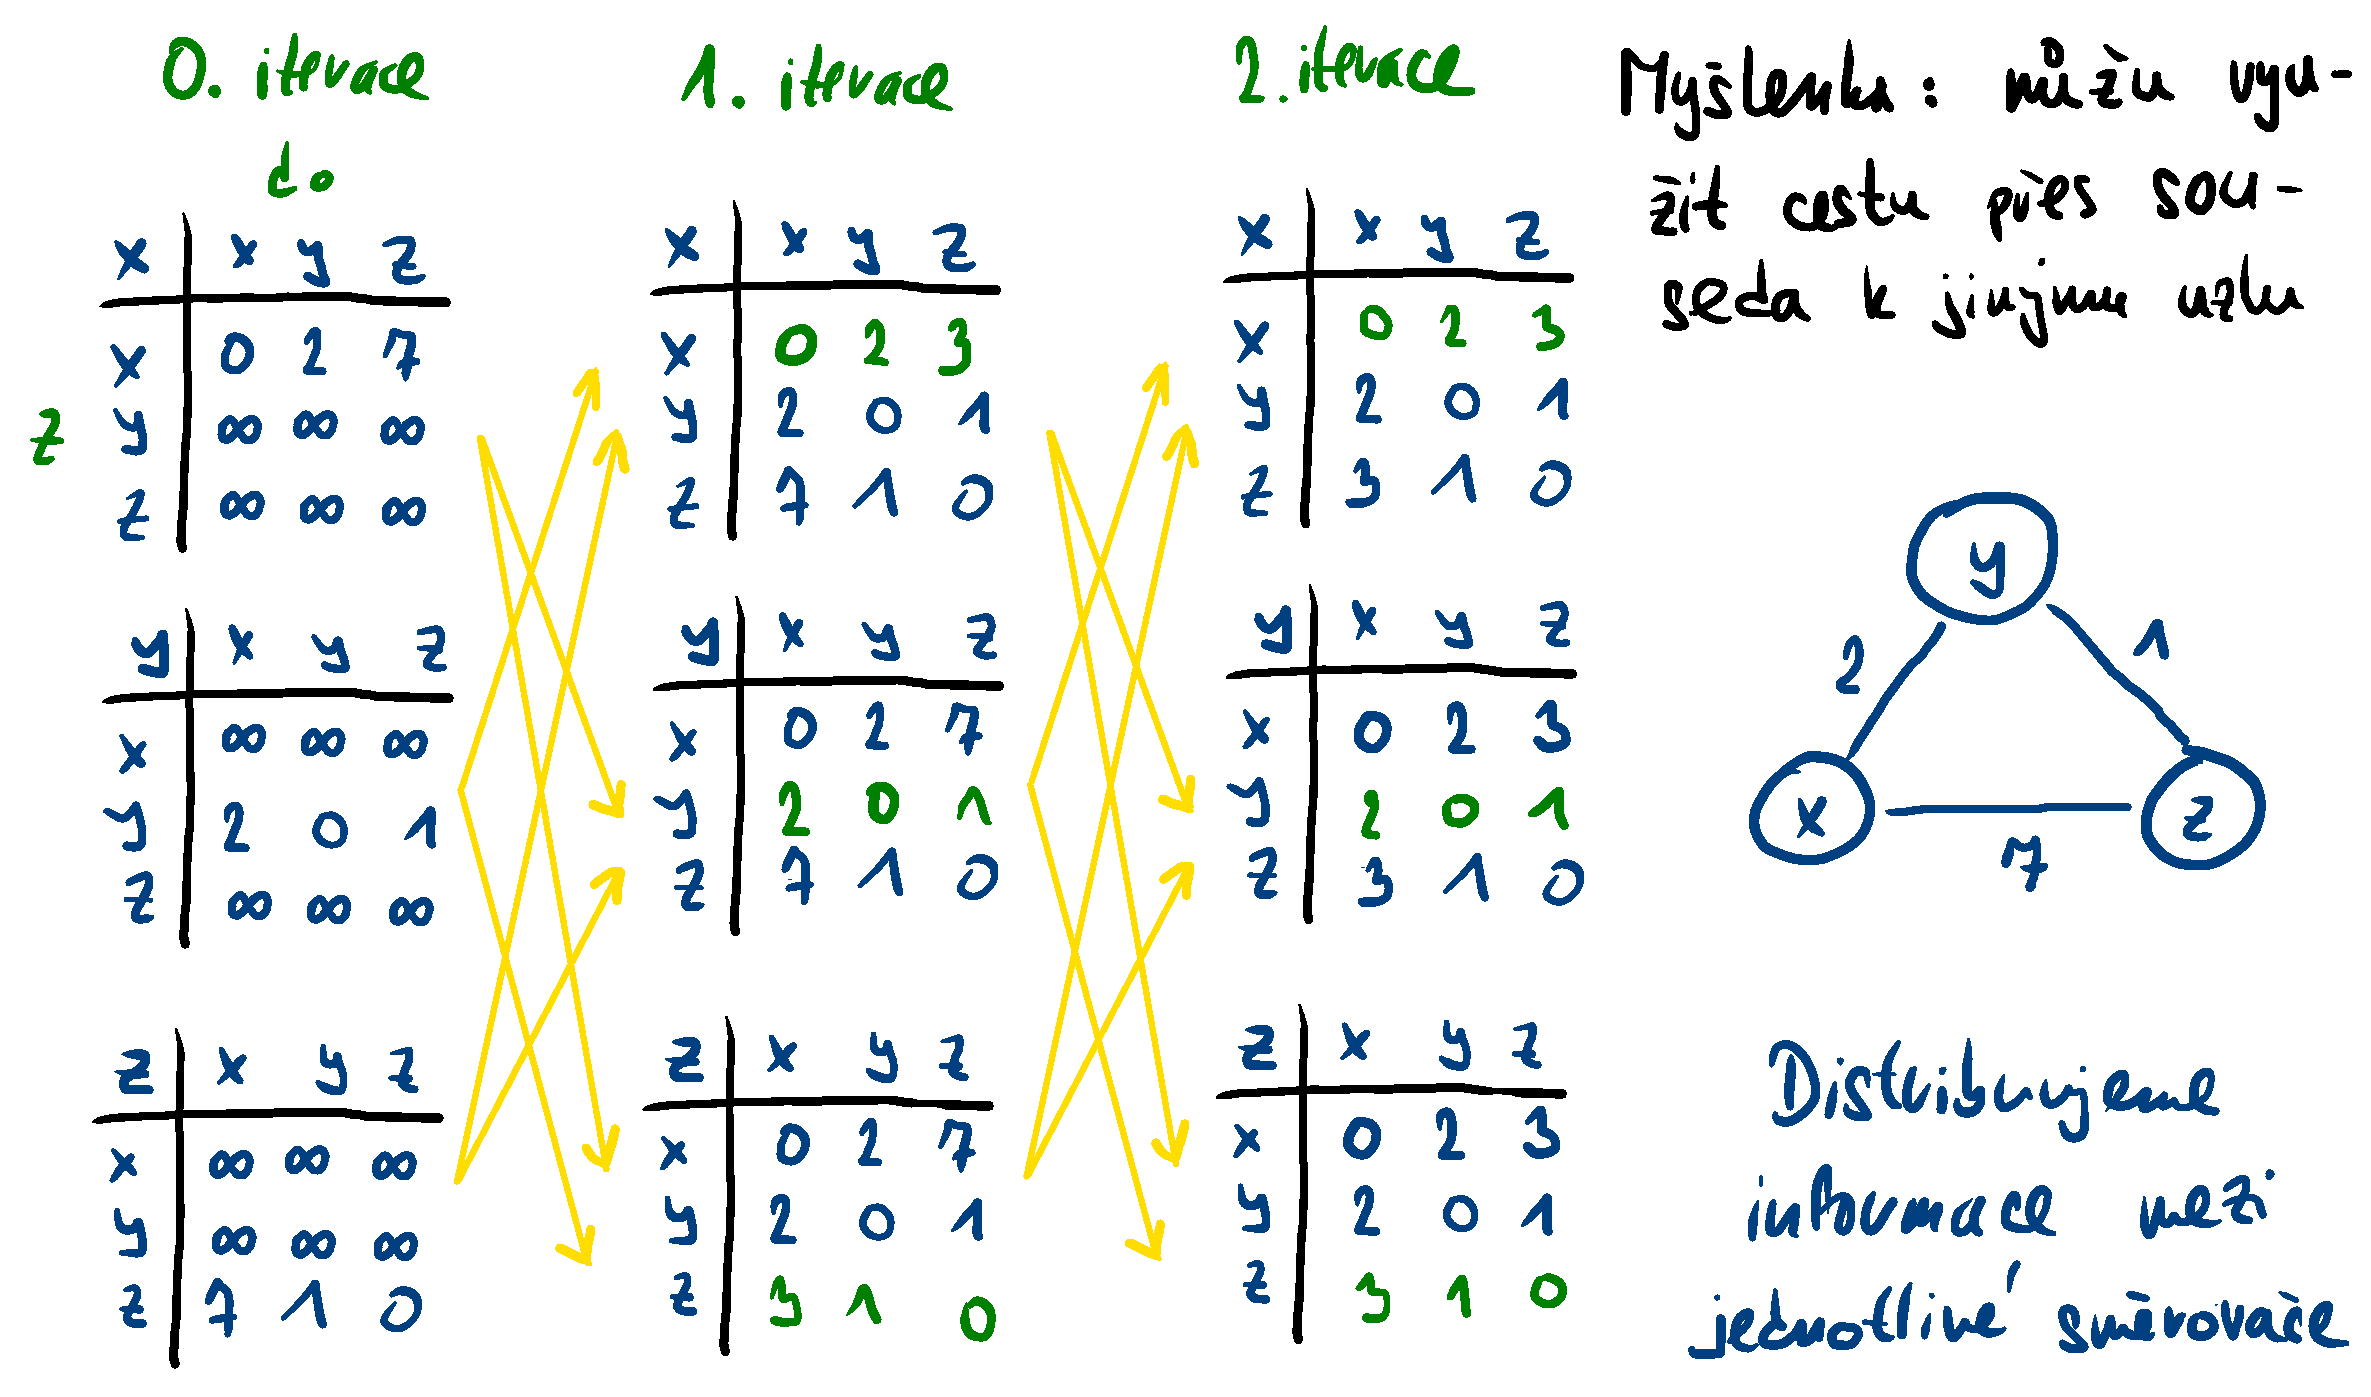
\includegraphics[width=1\linewidth]{bellman_ford_example.pdf}
    \caption{Příklad výpočtu nejkratší cesty pomocí algoritmu Bellman-Ford.}
\end{figure}

\paragraph*{Infinity Count} V případě, že vypadne některá ze sítí, může nastat problém počítání ceny cesty do nekonečna. Jelikož si uzly vyměňují pravidelně směrovací informace. Viz následující obrázek.

\begin{figure}[H]
    \centering
    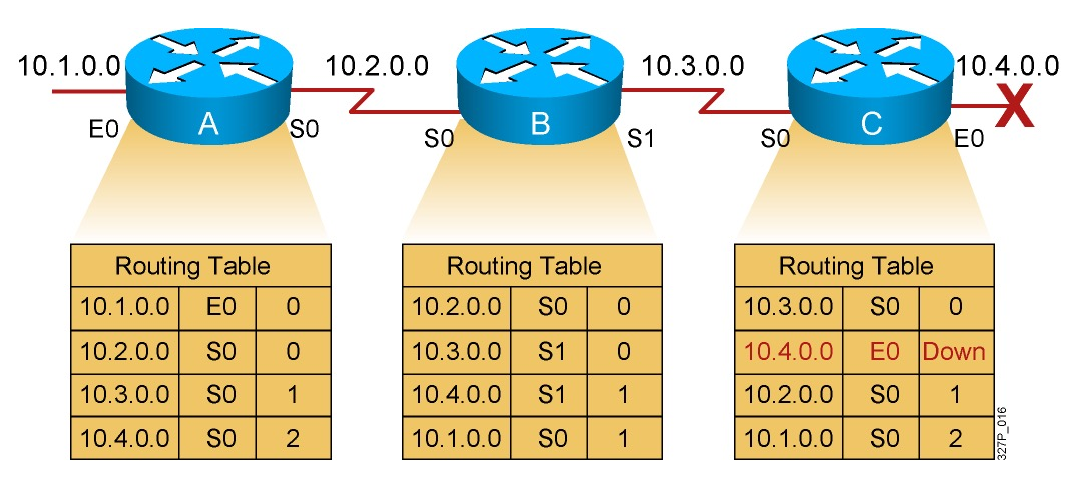
\includegraphics[width=1\linewidth]{rip_counting_infinity.pdf}
    \caption{Příklad \textit{Infinity Count}. Síť 10.4.0.0 vypadne a pro uzel C je najednou nedosažitelná. Uzel B se cestu do sítě 10.4.0.0 naučil dříve od C. Uzel C čerpá informaci o cestě do sítě z uzlu B. Tímto způsobem se cena do sítě zacyklí a jde k $\infty$.}
\end{figure}

\subsection{Diffusing update algorithm (DUAL)}

\begin{compactitem}
    \item Algoritmus DUAL (diffusing update algorithm) je algoritmus společnosti Cisco, který zajišťuje, že daná trasa je přepočítána globálně, kdykoli by mohla způsobit směrovací smyčku.
    \item Klíčová je tzv. \textbf{Feasibility Condition}, která zajišťuje, že jsou vždy vybírány pouze trasy bez smyček. Pokud podmínka platí, nemohou vzniknout žádné smyčky, ale podmínka může za určitých okolností odmítnout všechny trasy k cíli, přestože některé jsou bez smyček. \begin{compactitem}
        \item Vzdálenost sousedů k cílové síti nazveme RD (\textit{reported distance}).
        \item Nejlepší vzdálenost k danému uzlu nazveme FD (\textit{feasible distance}).
        \item Pokud platí $RD < FD$, tak cesta neobsahuje smyčku.
    \end{compactitem}
    \item Využívá jej směrovací protokol EIGRP (\textit{Enhanced Interior Gateway Routing Protocol}) od společnosti Cisco. \begin{compactitem}
        \item Pro hledání nejkratší cesty používá algoritmus Bellman-Ford + \textit{Feasibility Condition}.
        \item Komunikace: vlastní protokol zabalený do IP paketu (\textit{Reliable Transport Protocol}).
        \item Kompozitní metrika~--~jedno číslo spočítaný na základě několika parametrů (šířka pásma, zpoždění, rychlost, \dots).
    \end{compactitem}
\end{compactitem}

\begin{figure}[H]
    \centering
    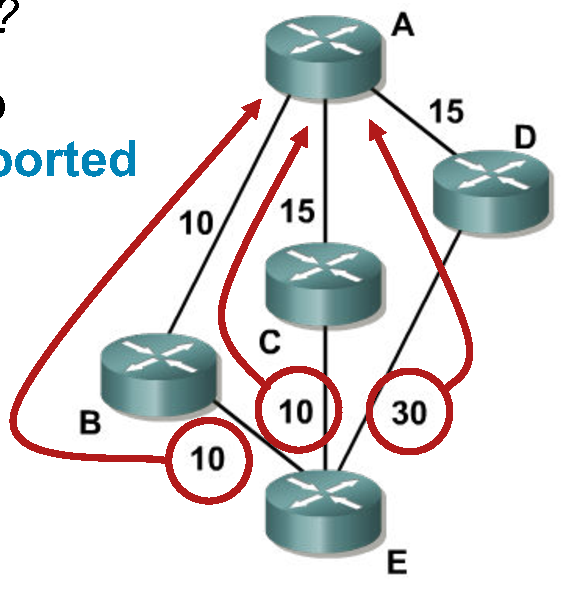
\includegraphics[width=0.4\linewidth]{feasibility_condition.pdf}
    \caption{Příklad výpočtu nejlepší cesty a uplatnění feasibility condition.}
\end{figure}

\noindent Cesta z A do E:
$$
RD(B) = 10 \;\;\;\;\;\;
RD(C) = 10 \;\;\;\;\;\;
RD(D) = 30
$$
$$
via(B) = 20 \;\;\;\;\;\;
via(C) = 25 \;\;\;\;\;\;
via(D) = 45
$$
Potom z pohledu A: \begin{compactitem}
    \item Cesta $via(B)$ je $FD$ a platí podmínka $FD > RD(B)$, tudíž cesta přes B neobsahuje smyčku.
    \item Pro cestu $via(C)$ platí podmínka $FD > RD(C)$, tudíž cesta přes C neobsahuje smyčku.
    \item Pro cestu $via(D)$ neplatí podmínka $FD > RD(D)$, tudíž cesta přes D může obsahovat smyčku a není brána v potaz.
\end{compactitem}

%%%%%%%%%%%%%%%%%%%%%%%%%%%%%%%%%%%%%%%%%%%%%%%%%%%%%%%%%%%%%%%%%%%%%%%%%%%%%%%%

\section{Link State přístup}

\begin{compactitem}
    \item Globální směrovací informace~--~Každý uzel zná celou topologii sítě. Na začátku si uzly vymění informace o topologii sítě.
    \item Používá se pro směrování uvnitř autonomních systémů.
    \item \textit{Single-metric}.
\end{compactitem}

\subsection{Dijkstrův algoritmus}

\begin{compactitem}
    \item \textit{Pro formální vysvětlení a pseudokód viz otázku \uv{Hledání nejkratších cest ze zdrojového uzlu do všech ostatních uzlů grafu}.}
    \item Jde o algoritmus hledání nejkratších cest ze zdrojového uzlu do všech ostatních uzlů. To znamená, že ho provádí každý uzel (směrovač).
    \item Používá ho např. směrovací protokol OSPF (\textit{Open Shortest Path First}). \begin{compactitem}
        \item Komunikace: vlastní protokol nad IP.
        \item Metrika: odvozena od rychlosti linky.
    \end{compactitem}
\end{compactitem}

\begin{figure}[H]
    \centering
    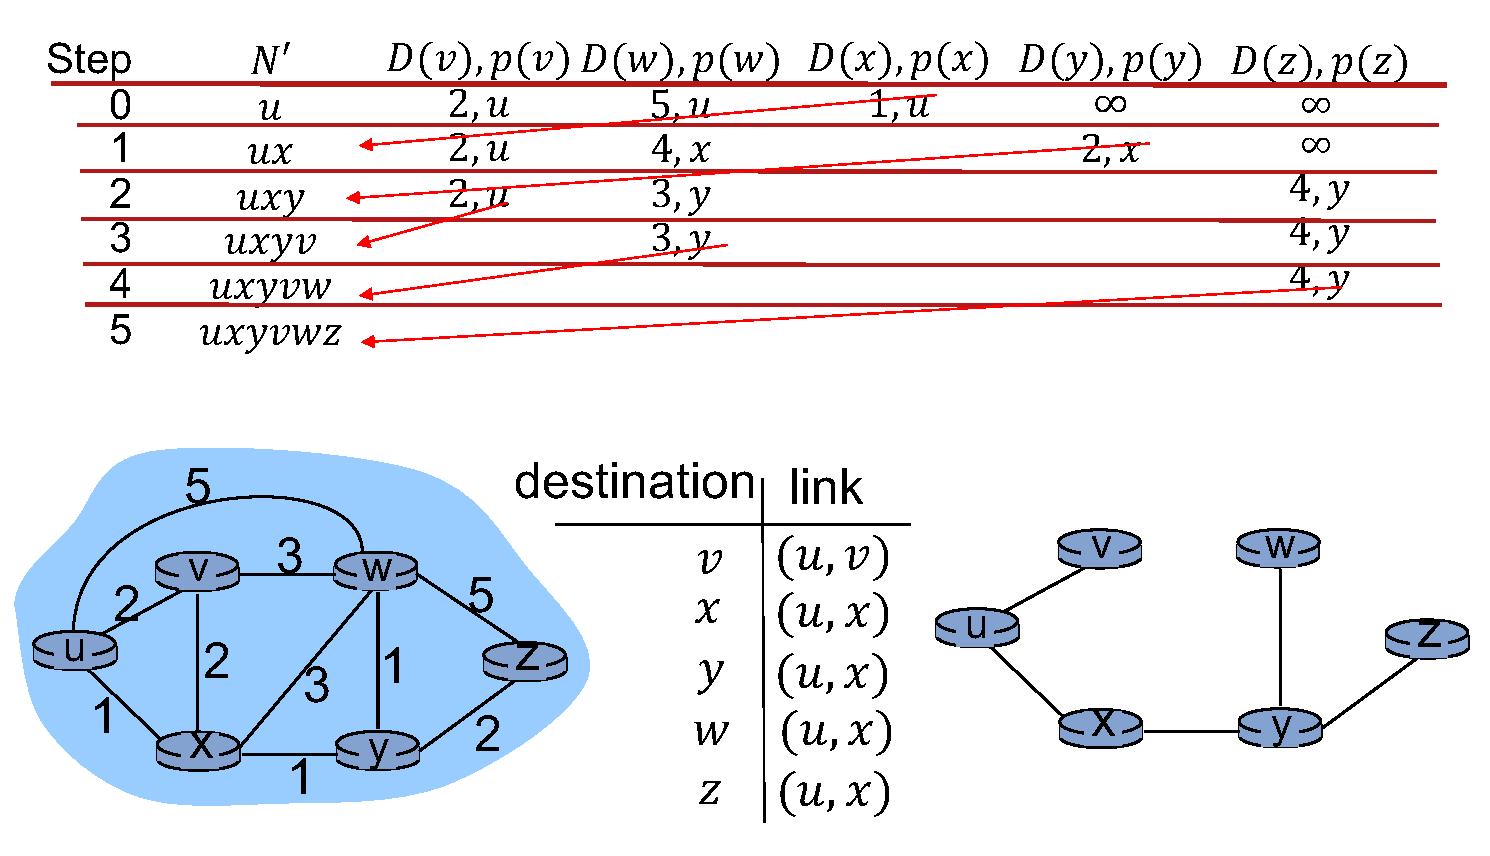
\includegraphics[width=1\linewidth]{dijkstra_example.pdf}
    \caption{Příklad výpočtu nejkratší cesty pomocí algoritmu Dijkstra. $Step$ značí iteraci, $N'$ je množina již prozkoumaných uzlů, $D$ je pole vzdáleností do uzlu, $p$ je pole předchůdzů uzlu.}
\end{figure}

%%%%%%%%%%%%%%%%%%%%%%%%%%%%%%%%%%%%%%%%%%%%%%%%%%%%%%%%%%%%%%%%%%%%%%%%%%%%%%%%

\section{Path Vector přístup}

\begin{compactitem}
    \item Globální směrovací informace.
    \item Na síť je pohlíženo jako na množinu autonomních systémů.
    \item Používá se pro směrování mezi autonomními systémy.
    \item \textit{Multi-metric}.
\end{compactitem}

\subsection{Path Vector algoritmus}

\begin{compactitem}
    \item Posílá celou cestu (posloupnost uzlů~--~autonomních systémů), ne jenom vzdálenost.
    \item Slouží také pro detekci smyček v rámci cesty.
    \item Cíl je projít přes co nejméně autonomních systémů.
    \item Umožňuje tzv. \textit{flexible policies}, můžu se rozhodnout jakou cestou budu provoz směrovat. Část provozu můžu přes $AS_1$, jinou část pres $AS_2$, apod.
    \item Známe celou cestu směrování, víme přes co pakety půjdou. \begin{compactitem}
        \item Můžeme část provozu posílat přes $AS_i$, jinou část provozu přes $AS_j$ apod.
        \item Nějakému $AS_i$ se můžeme chtít vyhnout na základě policies (horší parametry linky, horší cena).
    \end{compactitem}
    \item Směrovací protokol Border Gateway Protocol (BGP).
\end{compactitem}

\begin{figure}[H]
    \centering
    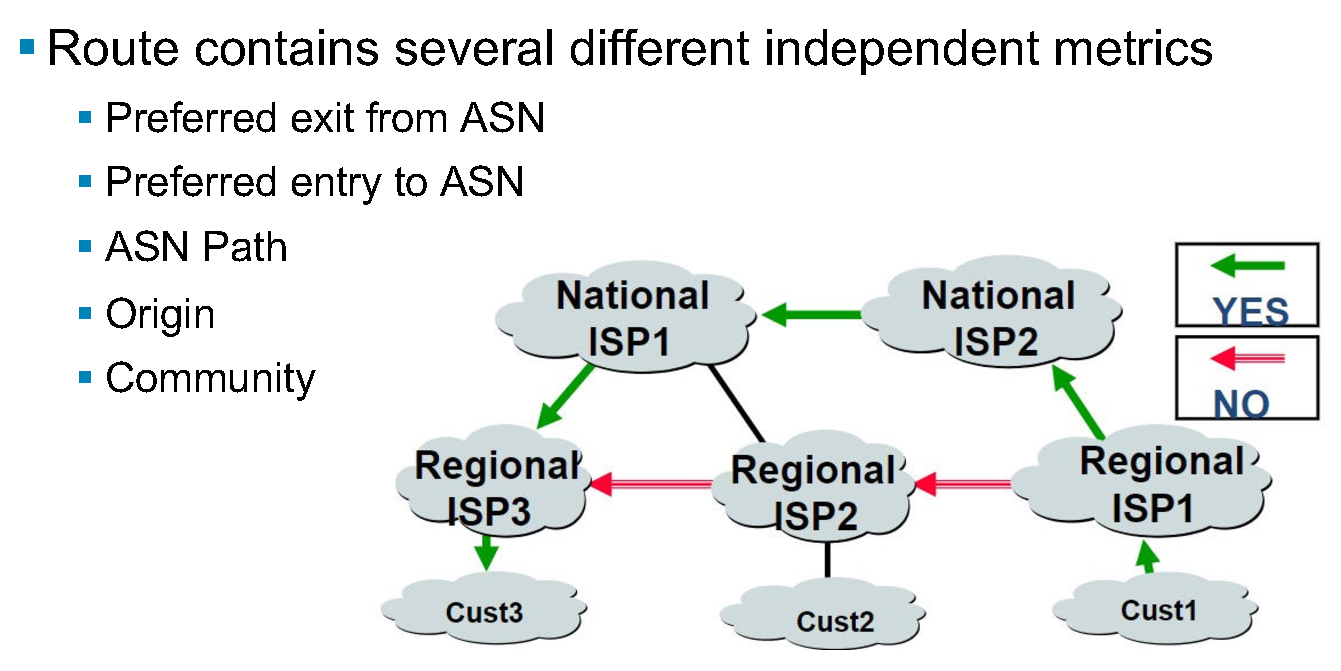
\includegraphics[width=0.75\linewidth]{path_vector.pdf}
    \caption{Path vector příklad.}
\end{figure}
